%
% File acl2018.tex
%
%% Based on the style files for ACL-2017, with some changes, which were, in turn,
%% Based on the style files for ACL-2015, with some improvements
%%  taken from the NAACL-2016 style
%% Based on the style files for ACL-2014, which were, in turn,
%% based on ACL-2013, ACL-2012, ACL-2011, ACL-2010, ACL-IJCNLP-2009,
%% EACL-2009, IJCNLP-2008...
%% Based on the style files for EACL 2006 by 
%%e.agirre@ehu.es or Sergi.Balari@uab.es
%% and that of ACL 08 by Joakim Nivre and Noah Smith

\documentclass[11pt,a4paper]{article}
\usepackage[hyperref]{acl2018}
\usepackage{times}
\usepackage{latexsym}
\usepackage{graphicx}

\usepackage{url}

\aclfinalcopy % Uncomment this line for the final submission
%\def\aclpaperid{***} %  Enter the acl Paper ID here

%\setlength\titlebox{5cm}
% You can expand the titlebox if you need extra space
% to show all the authors. Please do not make the titlebox
% smaller than 5cm (the original size); we will check this
% in the camera-ready version and ask you to change it back.

\newcommand\BibTeX{B{\sc ib}\TeX}

\title{Deliverable 2 - Summarization}

\author{Joshua Mathias \\
  University of Washington \\
  Seattle, WA \\
  {\tt emathias@uw.edu} 
  \\\And 
  Eric Lindberg \\
  U. of Washington \\
  Seattle, WA \\
  {\tt lindbe2@uw.edu} 
  \\\And 
  John Greve \\
  UW Linguistics Dept \\
  Seattle, WA \\
  {\tt jgreve@uw.edu } 
  \\\And 
  Kekoa Riggin \\
  UW \\
  Seattle, WA \\
  {\tt kekoar@uw.edu} 
    }

\date{}

\begin{document}
\maketitle

\section{System Overview}
This is the D2 system for Ling573 which establishes an end-to-end baseline summarization system. We read groups of stories and write extractive summaries to the outputs directory as specified by the D2 requirements. There are two methods for summarization: first sentence summarization (FSS) and pivoted QR matrix decomposition method for summarization (QRM). To evaluate we generate Rouge scores (Rouge 1-4) against provided gold standard summaries and discuss our baseline findings.

Operational Definitions: The requirements specified well-formed English sentences; for this deliverable we leave this to the level of syntax and punctuation. Semantic composition is outside of our scope.

\section{System Architecture}
The initial architecture diagram was mapped out as a UML class model (see Figure 1), highlighting the functional areas of the program we wanted to break into different components. In this diagram, the simple arrows mark usage or reference from one class to another. From this, it can be seen that the Summarizer module is the main controller, referring to most of the rest of the package.
\begin{figure}
\caption{UML diagram of summarization system}
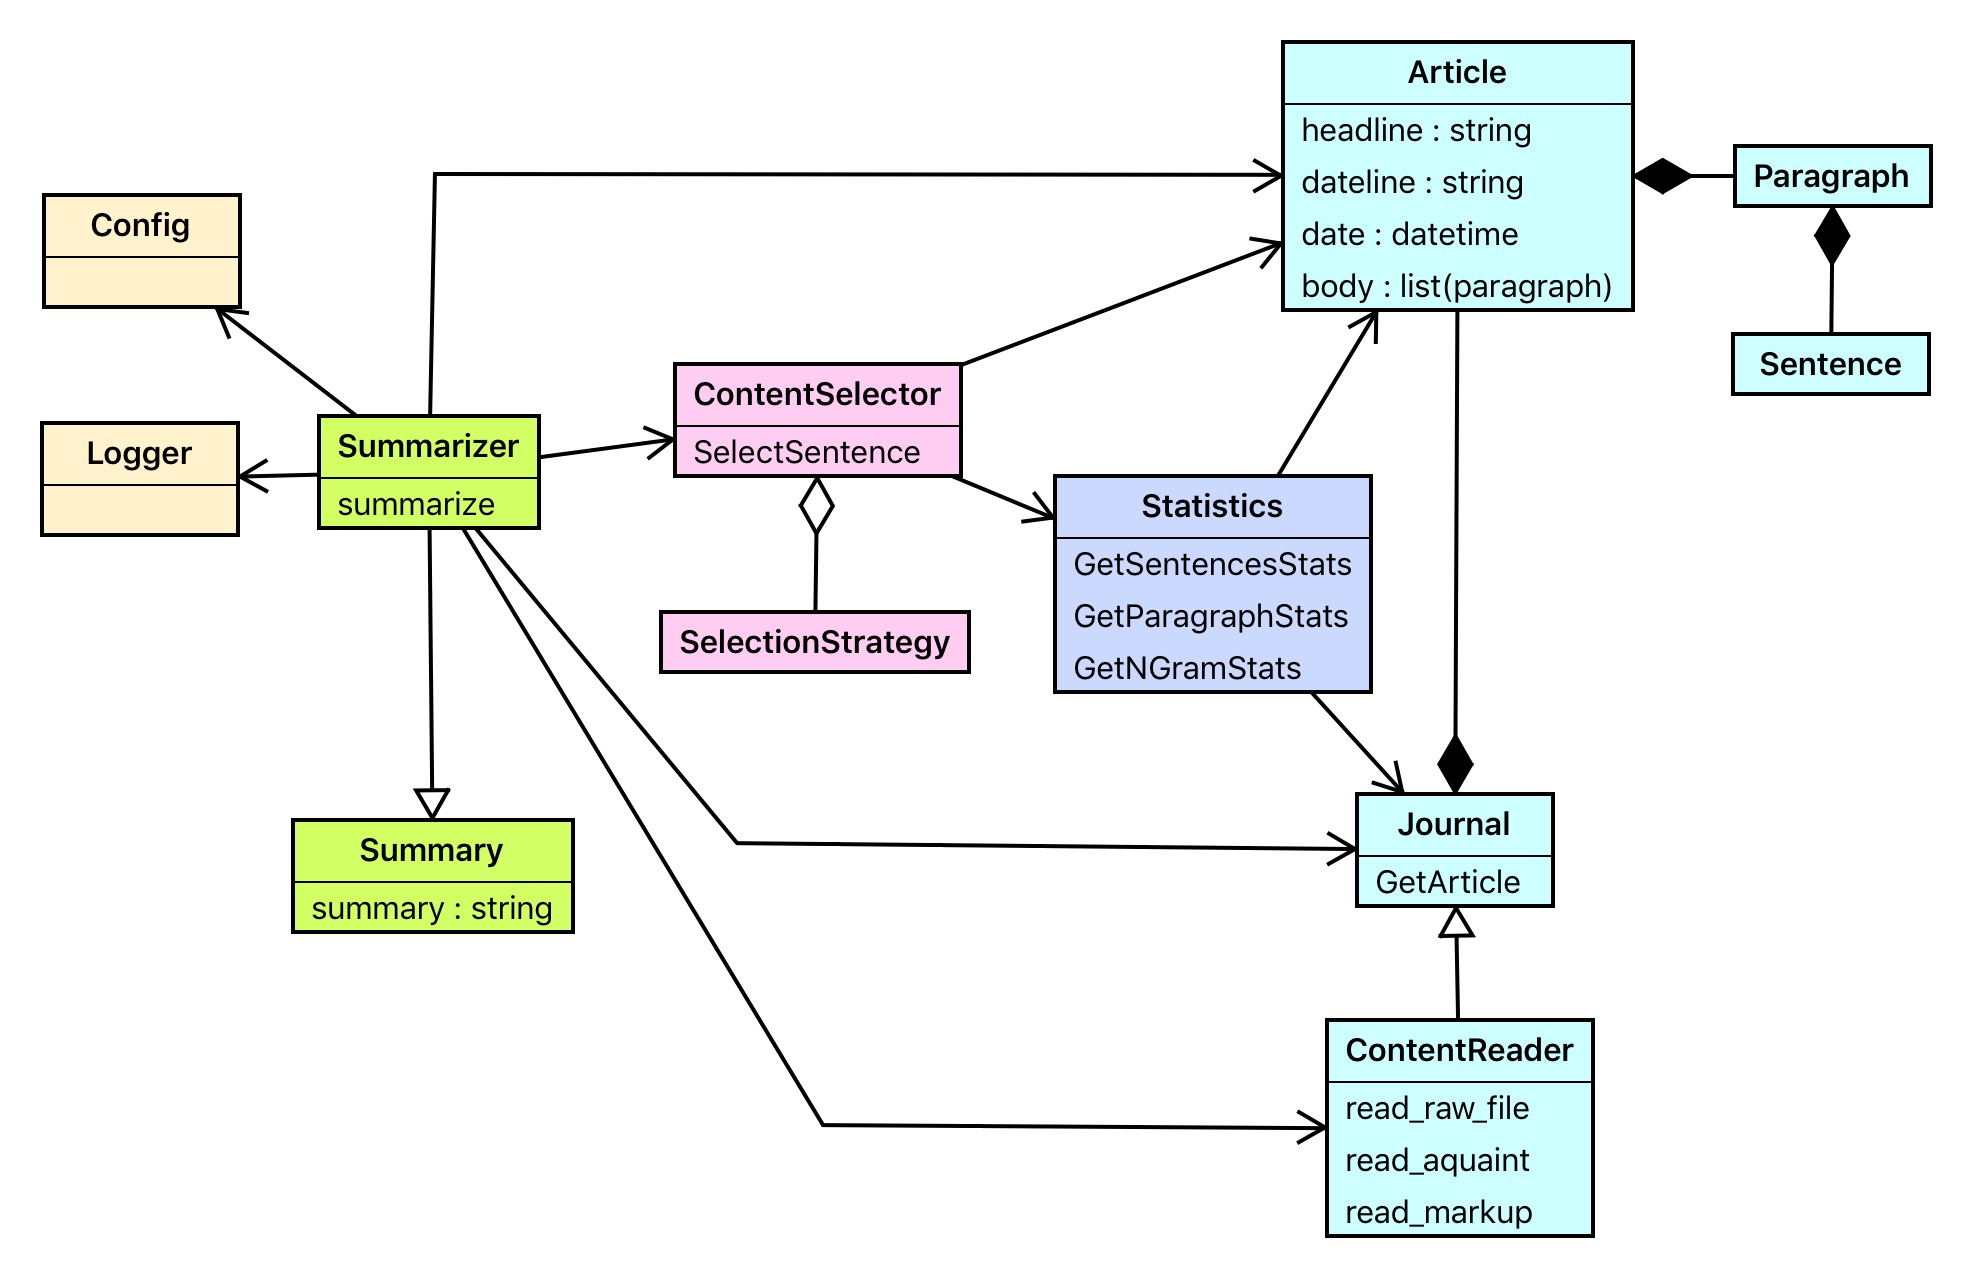
\includegraphics[width=80mm,scale=0.5]{architecture.png}
\end{figure}
In the final implementation, the Summarizer logic is contained in summarizer.py. Most of the ContentSelector is still in summarizer.py at this point, with fss.py and qrmatrix.py implementing the SelectionStrategy. The content\_provider.py module contains all of the ContentReader, Journal, and Article structures. Statistics are still gathered separately from the main program, for the most part, but will be expanded in the next release.\\
The unfilled triangular arrows mark generation, showing that the Summarizer creates summaries and that the ContentReader creates the Articles and Document Sets that the Summarizer operates on. Finally, the diamond connectors mark composition or collections, chiefly showing that a Document Set (or Journal) is made up of multiple Articles, which in turn are made up of Paragraphs composed of Sentences. The ContentSelector can refer to multiple selection strategies, though in retrospect this relationship might be one of subclassing rather than collection.\\
Ultimately, the components are divided into four general areas, Summarization, Data Gathering, Content Selection, and Statistics. These correspond roughly to a standard Model (Data Gathering), Controller (Content Selection and Statistics), View (Summarization) structure.\\

\section{Approach}
The system is capable of single- and multi-document summarization and can handle batch processing. 

For each document group in a batch, we read the data from the specified source, as detailed in a configuration file; select sentences to extract for the summary; compile the sentences into the realized summary; and write summary to output files.

Then scoring is applied using the reference implementation for this project.

\subsection{Content Selection}
Our current system features two methods for summarization. The first is a first sentence summarization and the second is a pivoted QR matrix decomposition. 

FSS means that the first sentence of each article in a docset is selected. Given the nature of news articles, this approach produces a fair summary with very little processing.

The pivoted QR matrix decomposition approach, uses feature vectors, based on the sentences in a docset ~\cite{Conroy:01}. Said feature vectors comprise a matrix, where each row represents a sentence and each column represents a feature. In the Conroy paper, these features are meant to capture ideas, which are represented by the words in each sentence. 

The sum of each feature vector is weighted, using a weighting function from the paper. This weighted sum is the score for each sentence. The sentence with the highest score is selected. Then, the features from that sentence are removed from the matrix. This reduces redundancy in future sentences that will be selected. 

Once all features from the selected sentence have been removed from the remaining feature vectors, the sentence scores are recalculated and this process is repeated until no more sentences will fit in the 100-word summary.

If the best scoring sentence at any recursion of the matrix is too long to add to the summary, the next best scoring sentence that is not too long is used. 

\subsection{Information Ordering}
For our baseline FSS method sentences are simply used in the same order that each article is processed.

In our QRM method, sentences that appear earlier in their article appear earlier in our summary. This means that a selected sentence that has a high score may appear lower in the summary while a lower score may appear higher. The goal of this feature is to allow descriptive sentences near the beginning of a news article to appear before sentences that explain or expound later in their own articles. 

This ordering decision has no effect on the ROUGE score for our summaries, but we subjectively believe that this ordering affects their readability.

\subsection{Content Realization}
To generate the summary, we look at each selected sentence sequentially. If the sum of the words in the summary and the words in the current selected sentence is less than 100, the sentence is added to the summary. This realization strategy isn’t particularly clever, but it does ensure that the summary adheres to the length requirement and contains only complete sentences. We chose to exclude sentences of less than six words.

Each summary is written to a summary file formatted as described in the Delivery 2 specifications.

\section{Results}
Here we present our baseline results. The two summarization strategies we tried are FSS Scores and QRM Scores. Since recall and precision appear correlated the F-Scores track with them. This indicates we are not suffering anomalies from excellent recall at the expense of precision or vice-versa. We observed consistently higher FSS Scores over QRM Scores.\\

\begin{table}[h]
\centering
\caption{Average FSS Scores}
\label{table1}
\begin{tabular}{|l|l|l|l|}
\hline
Averages   & RECALL  & PREC    & F-SCORE \\ \hline
ROUGE-1    & 0.21842 & 0.23413 & 0.22481 \\ \hline
ROUGE-2    & 0.05359 & 0.05758 & 0.05521 \\ \hline
ROUGE-3    & 0.01612 & 0.01747 & 0.01669 \\ \hline
ROUGE-4    & 0.00455 & 0.00498 & 0.00473 \\ \hline
\end{tabular}
\end{table}

\begin{table}[h]
\centering
\caption{Average QRM Scores}
\label{table2}
\begin{tabular}{|l|l|l|l|}
\hline
Averages & RECALL  & PREC    & F-SCORE \\ \hline
ROUGE-1  & 0.16196 & 0.20005 & 0.17844 \\ \hline
ROUGE-2  & 0.03677 & 0.04512 & 0.04039 \\ \hline
ROUGE-3  & 0.01115 & 0.01391 & 0.01234 \\ \hline
ROUGE-4  & 0.00279 & 0.00348 & 0.00309 \\ \hline
\end{tabular}
\end{table}

In Figure 2 you can more easily see the difference between FSS and QRM. It is striking that the ROUGE-1 scores are so much higher than the other rouge scores.

\begin{figure}
\caption{Average ROUGE-n RECALL for QMR and FSS (N=46 doc sets)}
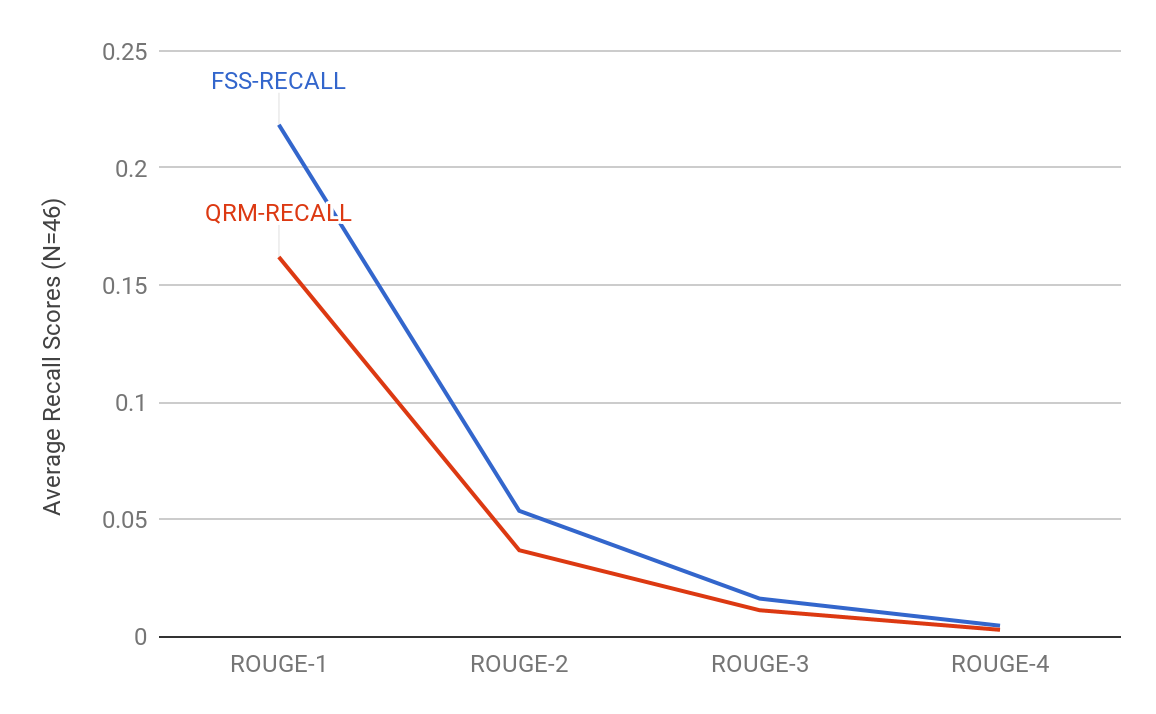
\includegraphics[width=80mm,scale=0.5]{rouge_graph.png}
\end{figure}

\section{Discussion}
While we were impressed at how well the FSS strategy work we were also surprised at how quickly the rouge scores dropped off. Table 3 shows counts of zero FSS Recall scores for the actual documents. Interestingly everything in ROUGE-1 were able to recall something (e.g. no zero counts). QRM received proportionally similar results and is omitted for brevity.

\begin{table}[h]
\centering
\caption{FSS Percentage of Zero Scores}
\label{table3}
\begin{tabular}{|l|l|l|l|l|}
\hline
& ROUGE-1 & R2 & R3 & R4 \\ \hline
\#    & 0       & 3       & 14      & 33      \\ \hline
\%   & 0.00\%  & 6.52\%  & 30.43\% & 71.74\% \\ \hline
\end{tabular}
\end{table}

To drill into this a little further we are including a heat-map style representation of the observed FSS scores (Figure 3). The reason is that larger N-gram matches become increasingly rare as we go from ROUGE-1 up to ROUGE-4. This will motivate us to look closer into various gold standard N-grams and sample which ones performed well in our baseline and compare them with which ones were absent from our baseline.

\begin{figure}
\caption{ROUGE heat map for FSS}
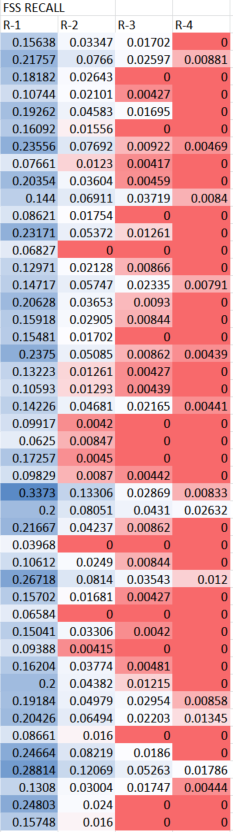
\includegraphics[width=80mm,height=240mm,scale=0.1]{rouge_heat_map.png}
\end{figure}

This finding shows that we are missing scores, which suggests that the number of empty values will be one of the focuses of our research.

The important thing isn't numeric values but the patterns of zeros (darker red). This pattern will guide the specific doc sets we sample to understand what n-grams matched well in ROUGE scoring for our initial summarization and what matched worse, as in not at all.

We anticipate finding a number of surface features (punctuation, space formatting and so on) that will increase ROUGE scores against the gold standards. We also expect that the missing longer n-grams will yield direction for where to focus our summarization efforts.

In analyzing our system’s results, we realized that we had overlooked the normalization of our feature vectors in terms of punctuation and capitalization. We cannot speak to the significance of the impact this lack of normalization had on our ROUGE scores, but we anticipate improved performance from our system once  our QRM method features normalization for punctuation and capitalization.

% ~\cite{Du:12}
% ~\cite{Lau:17}
% \textbf{Citations}: Citations within the text appear in parentheses
% itself, as Gusfield~\shortcite{Gusfield:97}.
% Using the provided \LaTeX\ style, the former is accomplished using
% {\verb|\cite|} and the latter with {\verb|\shortcite|} or {\verb|\newcite|}.

% \subsection{Equation}
% \label{ssec:eqn}

% \begin{equation}
% A=\pi r^2
% \end{equation}


%Here we give a simple criterion on your colored figures, if your paper has to be printed in black and white, then you must assure that every curves or points in your figures can be still clearly distinguished.

% Min: no longer used as of ACL 2017, following ACL exec's decision to
% remove this extra workflow that was not executed much.
% BEGIN: remove
%% \section{XML conversion and supported \LaTeX\ packages}

%% Following ACL 2014 we will also we will attempt to automatically convert 
%% your \LaTeX\ source files to publish papers in machine-readable 
%% XML with semantic markup in the ACL Anthology, in addition to the 
%% traditional PDF format.  This will allow us to create, over the next 
%% few years, a growing corpus of scientific text for our own future research, 
%% and picks up on recent initiatives on converting ACL papers from earlier 
%% years to XML. 

%% We encourage you to submit a ZIP file of your \LaTeX\ sources along
%% with the camera-ready version of your paper. We will then convert them
%% to XML automatically, using the LaTeXML tool
%% (\url{http://dlmf.nist.gov/LaTeXML}). LaTeXML has \emph{bindings} for
%% a number of \LaTeX\ packages, including the ACL 2017 stylefile. These
%% bindings allow LaTeXML to render the commands from these packages
%% correctly in XML. For best results, we encourage you to use the
%% packages that are officially supported by LaTeXML, listed at
%% \url{http://dlmf.nist.gov/LaTeXML/manual/included.bindings}
% END: remove



% include your own bib file like this:
%\bibliographystyle{acl}
%\bibliography{acl2018}
\bibliography{acl2018}
\bibliographystyle{acl_natbib}
% \appendix


\end{document}

